\ylDisplay{Õhupalli vari} % Ülesande nimi
{Jaan Kalda} % Autor
{lahtine} % Voor
{2013} % Aasta
{G 10} % Ülesande nr.
{10} % Raskustase
{
% Teema: Varia
\ifStatement
Päikesepaistelisel päeval hõljub õhus kerakujuline läbipaistmatu õhupall, mis
jätab horisontaalsele maapinnale varju, kusjuures poolvarju pikkus on \SI{5,0}{m}
ja laius \SI{2,5}m ning täisvarju pikkus \SI{1,0}{m}. Kui suur on palli
läbimõõt ja kui kõrgel see on maapinnast? Päikese näiv nurkläbimõõt  (see on nurk, 
mis moodustub kahe kiire vahel, mis on tõmmatud vaatleja silma juurest 
Päikese diameetri otspunktide juurde) oli sel
päeval $\alpha =0,53^\circ$.
\fi


\ifHint
Kuna täisvari on poolvarjust märksa väiksem ja Päikese nurkläbimõõt on ka väike, peab õhupall maapinnast suhteliselt kaugel olema. Seega võib maapinna läheduses lugeda varju koonuseid ligikaudu silindriteks. Paneme tähele, et poolvarju koonuse läbimõõt maapinna läheduses on \SI{2,5}{m}, sest poolvarju laius (väikseim mõõde) vastab koonuse läbimõõdule. Analoogselt on täisvarju koonuse läbimõõt $\SI{1,0}{m}\cdot\frac{\SI{2,5}{m}}{\SI{5,0}{m}} = \SI{0,5}{m}$.
\fi


\ifSolution
Et Päikese nurksuurus on väike, siis maapinna lähedal võime lugeda varjukoonused silindriteks: joonisel tähendab see, et loeme $AH$ paralleelseks $DG$-ga, $CF$-ga ja $BE$-ga.
Paneme tähele, et $|AD|=\SI{2,5}m$, sest kaldu langevate kiirte puhul on kera varju laius (väiksem mõõde) maapinnal võrdne varjukoonuse läbimõõduga.
See tähendab, et $CB$ pikkus on \SI{0,5}m ja $AB$ pikkus on $\frac{2,5-0,5}2\SI{}m=\SI{1}m$. Et palli läbimõõt on võrdne $AC$-ga, siis $|KL|=1+0,5\SI{}m=\SI{1,5}m$.
Nurk $\angle KJL$ moodustab sirgnurgast murdosa $0,5/180=\frac 1{360}$, mis tähendab, et lõik $KL$ moodustab punkti $J$ ümber tõmmatud poolringjoonest raadiusega $R=|JK|$
samasuguse murdosa; selle kaare pikkus on $\pi R$, st $|KL|=\pi R /360$, millest $R=360|KL|/\pi\approx \SI{172}m$. Sarnastest kolmnurkadest $JKL$ ja $JBC$ leiame, et $|BK|=|JK|\frac{|KL|-|BC|}{|KL|}\approx \SI{114}m$. Ligikaudu sarnastest kolmnurkadest $KAM$ ja $ADG$ leiame, et  $|KM|\approx |KA|\frac{|DA|}{|AG|}\approx \SI{57}m$.

\begin{center}
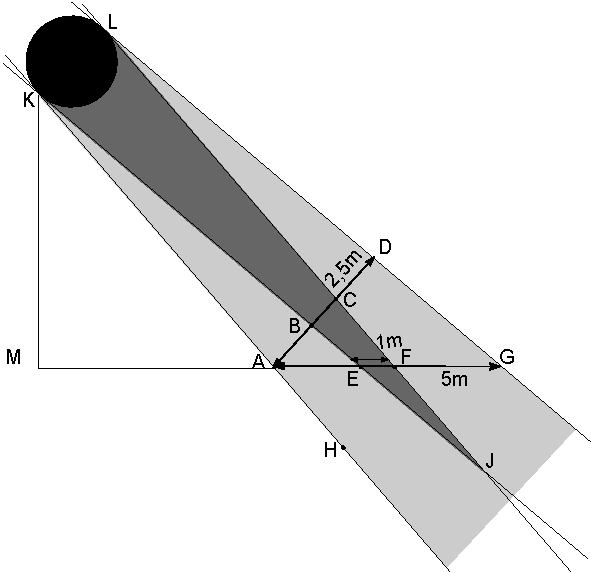
\includegraphics[width=250pt]{2013-lahg-10-pxike-pall-vari}%
\end{center}
\fi


\ifEngStatement
% Problem name: Shadow of a balloon
A spherical opaque balloon is floating during a sunny day and leaves a shadow on a horizontal ground, moreover the length of the penumbra is 5.0 m and the width 2.5 m and the length of the umbra is 1.0 m. How big is the diameter of the ball and how high is it from the ground? The apparent angular diameter of the Sun (the angle that forms between the two lines that are drawn from the eye of the observer to the ends of the Sun’s diameter) was $\alpha =0.53^\circ$ during that day.
\fi


\ifEngHint
Because the umbra is considerably smaller than the penumbra and the angular diameter of the Sun is small then the balloon has to be quite far from the ground. Thus, the cones of shadows near the ground can be assumed to be as approximately cylinders. Let us notice that the diameter of the penumbra’s cone near the ground is 2.5 m because the width (smaller dimension) of the penumbra corresponds to the diameter of the cone. Similarly the diameter of the umbra’s cone is $\SI{1,0}{m}\cdot\frac{\SI{2,5}{m}}{\SI{5,0}{m}} = \SI{0,5}{m}$.
\fi


\ifEngSolution
Since the Sun's angular velocity is small then close to the ground we can assume the shadow cones to be cylinders: in the figure it means that we assume $AH$ to be parallel to $DG$, $CF$ and $BE$. Let us notice that $|AD|=\SI{2,5}m$ because in the case of inclined rays the width (the smaller dimension) of the sphere's shadow on the ground is equal to the shadow cone's diameter. This means that the section's $CB$ length is 0.5 m and the section's $AB$ length is $\frac{2,5-0,5}2\SI{}m=\SI{1}m$. Since the ball's diameter is equal to $AC$ then $|KL|=1+0,5\SI{}m=\SI{1,5}m$. The angle $\angle KJL$ forms a fraction $0,5/180=\frac 1{360}$ of the flat angle, which means that the section $KL$ forms the same fraction of the half circle with a radius $R=|JK|$ that is drawn around the point $J$; the length of this arc is $\pi R$, meaning $|KL|=\pi R /360$ from which $R=360|KL|/\pi\approx \SI{172}m$. From similar triangles $JKL$ and $JBC$ we find that $|BK|=|JK|\frac{|KL|-|BC|}{|KL|}\approx \SI{114}m$. From approximately similar triangles $KAM$ and $ADG$ we find that $|KM|\approx |KA|\frac{|DA|}{|AG|}\approx \SI{57}m$.
\begin{center}
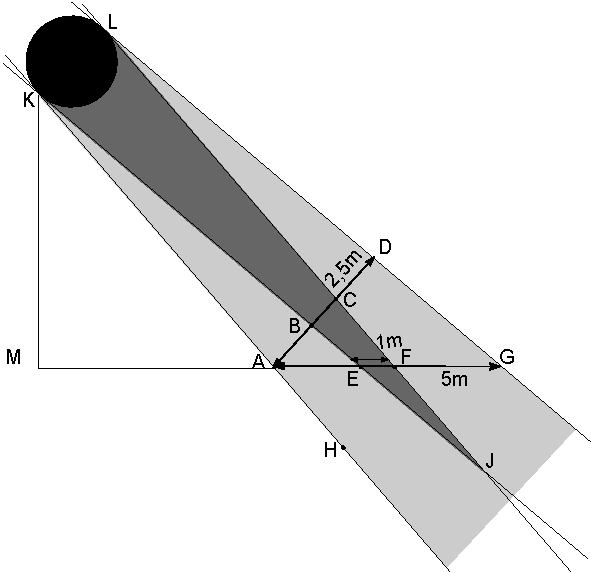
\includegraphics[width=250pt]{2013-lahg-10-pxike-pall-vari}%
\end{center}
\fi
}